\documentclass{../ucll-slides}
\usepackage{pxfonts}
\usepackage{tikz}
\usepackage{calc}
\usepackage{../ucll-code}


\usetikzlibrary{calc,shadows,tikzmark}

\coursename{Distributed Applications}
\title{Linked Lists}



\begin{document}

\maketitle

\section{Arrays}

\begin{frame}
    \frametitle{Arrays}
    \begin{center}
        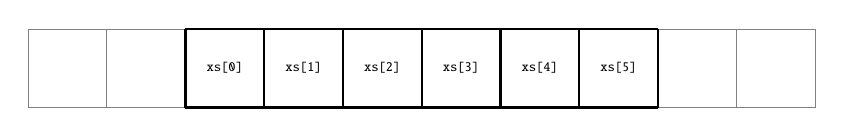
\begin{tikzpicture}
            \draw[help lines] (-2,0) grid (8,1);
            \draw[thick] (0,0) grid (6,1);
            \foreach \x in {0,...,5} {
                \node[font=\tiny] at ($ (\x,0.5) + (0.5,0) $) { \texttt{xs[\x]} };
            }
        \end{tikzpicture}
    \end{center}
    \vskip4mm
    \structure{Memory Layout}
    \begin{itemize}
        \item One piece of contiguous memory
    \end{itemize}
    \vskip4mm
    \structure{Fast Operations}
    \begin{itemize}
        \item Querying length
        \item Reading/overwriting element at index \texttt{i}
    \end{itemize}
    \vskip4mm
    \structure{Slow Operations}
    \begin{itemize}
        \item Inserting or removing an element requires copying
    \end{itemize}
\end{frame}

\section{Linked Lists}

\begin{frame}
    \frametitle{Linked Lists}
    \begin{center}
        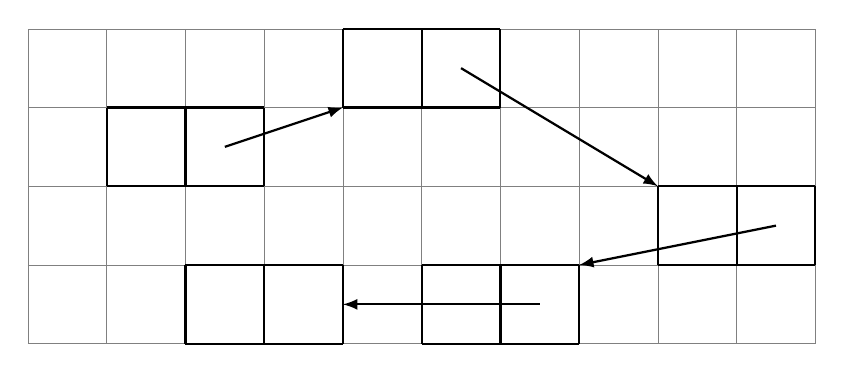
\begin{tikzpicture}[link/.style={thick,-latex}]
            \draw[help lines] (0,0) grid (10,4);
            \draw[thick] (1,2) grid ++(2,1);
            \draw[thick] (4,3) grid ++(2,1);
            \draw[thick] (5,0) grid ++(2,1);
            \draw[thick] (2,0) grid ++(2,1);
            \draw[thick] (8,1) grid ++(2,1);

            \draw[link] (2.5,2.5) -- (4,3);
            \draw[link] (5.5,3.5) -- (8,2);
            \draw[link] (9.5,1.5) -- (7,1);
            \draw[link] (6.5,0.5) -- (4,0.5);
        \end{tikzpicture}
    \end{center}
    \vskip4mm
    \structure{Memory Layout}
    \begin{itemize}
        \item List consists of series of nodes
        \item Each node has two fields
              \begin{itemize}
                \item Item
                \item Reference to next node
              \end{itemize}
        \item Nodes spread across memory
    \end{itemize}
\end{frame}

\begin{frame}
    \frametitle{Linked Lists in Code}
    \code[language=csharp]{LinkedList.cs}
\end{frame}

\begin{frame}
    \frametitle{Created a Linked List}
    \begin{center}
        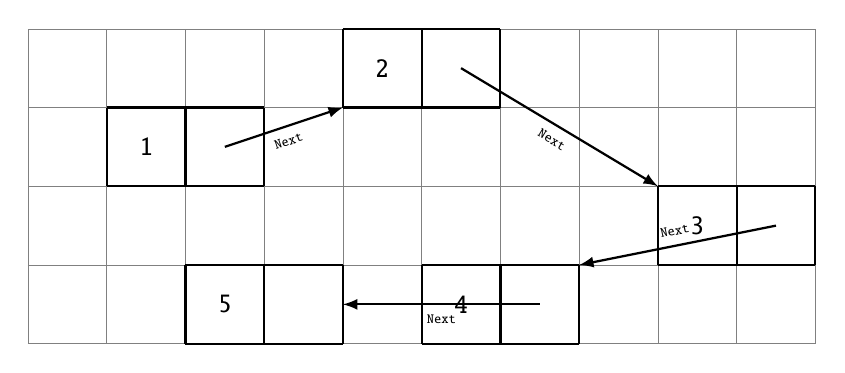
\begin{tikzpicture}[link/.style={thick,-latex}]
            \draw[help lines] (0,0) grid (10,4);
            \draw[thick] (1,2) grid ++(2,1);
            \draw[thick] (4,3) grid ++(2,1);
            \draw[thick] (5,0) grid ++(2,1);
            \draw[thick] (2,0) grid ++(2,1);
            \draw[thick] (8,1) grid ++(2,1);

            \draw[link] (2.5,2.5) -- (4,3) node[midway,font=\tiny\ttfamily,sloped,below]{Next};
            \draw[link] (5.5,3.5) -- (8,2) node[midway,font=\tiny\ttfamily,sloped,below]{Next};
            \draw[link] (9.5,1.5) -- (7,1) node[midway,font=\tiny\ttfamily,sloped,above]{Next};
            \draw[link] (6.5,0.5) -- (4,0.5) node[midway,font=\tiny\ttfamily,sloped,below]{Next};

            \node[font=\ttfamily] at (1.5,2.5) {1};
            \node[font=\ttfamily] at (4.5,3.5) {2};
            \node[font=\ttfamily] at (8.5,1.5) {3};
            \node[font=\ttfamily] at (5.5,0.5) {4};
            \node[font=\ttfamily] at (2.5,0.5) {5};
        \end{tikzpicture}
    \end{center}
    \vskip4mm
    \code[language=csharp]{LinkedListCreation.cs}
\end{frame}

\begin{frame}
    \frametitle{Determining Length}
    \begin{center}
        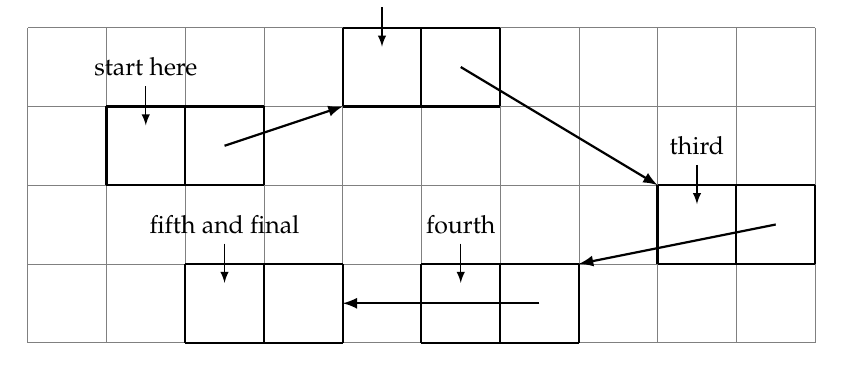
\begin{tikzpicture}[link/.style={thick,-latex}]
            \path[use as bounding box] (0,0) rectangle (10,4);

            \coordinate (p1) at (1, 2);
            \coordinate (p2) at (4, 3);
            \coordinate (p3) at (8, 1);
            \coordinate (p4) at (5, 0);
            \coordinate (p5) at (2, 0);

            \draw[help lines] (0,0) grid (10,4);
            \draw[thick] (p1) grid ++(2,1);
            \draw[thick] (p2) grid ++(2,1);
            \draw[thick] (p3) grid ++(2,1);
            \draw[thick] (p4) grid ++(2,1);
            \draw[thick] (p5) grid ++(2,1);

            \draw[link] (2.5,2.5) -- (4,3);
            \draw[link] (5.5,3.5) -- (8,2);
            \draw[link] (9.5,1.5) -- (7,1);
            \draw[link] (6.5,0.5) -- (4,0.5);

            \foreach \k/\label in {1/{start here},2/{second},3/{third},4/{fourth},5/{fifth and final}} {
                \only<\k>{
                    \node[font=\small] (tag) at ($ (p\k) + (0.5,1.5) $) { \label };
                    \draw[-latex] (tag.south) -- ++(0,-0.5);
                }
            }
        \end{tikzpicture}
    \end{center}
    \vskip4mm
    \structure{Algorithm}
    \begin{itemize}
        \item Follow nodes until we find \texttt{null}
        \item Count number of jumps necessary
        \item Takes longer for longer lists
    \end{itemize}
\end{frame}

\end{document}

%%% Local Variables:
%%% mode: latex
%%% TeX-master: t
%%% End:
